%File: anonymous-submission-latex-2024.tex
\documentclass[letterpaper]{article} % DO NOT CHANGE THIS
\usepackage[submission]{aaai24}  % DO NOT CHANGE THIS
\usepackage{times}  % DO NOT CHANGE THIS
\usepackage{helvet}  % DO NOT CHANGE THIS
\usepackage{courier}  % DO NOT CHANGE THIS
\usepackage[hyphens]{url}  % DO NOT CHANGE THIS
\usepackage{graphicx} % DO NOT CHANGE THIS
\urlstyle{rm} % DO NOT CHANGE THIS
\def\UrlFont{\rm}  % DO NOT CHANGE THIS
\usepackage{natbib}  % DO NOT CHANGE THIS AND DO NOT ADD ANY OPTIONS TO IT
\usepackage{caption} % DO NOT CHANGE THIS AND DO NOT ADD ANY OPTIONS TO IT
\frenchspacing  % DO NOT CHANGE THIS
\setlength{\pdfpagewidth}{8.5in} % DO NOT CHANGE THIS
\setlength{\pdfpageheight}{11in} % DO NOT CHANGE THIS
%
% These are recommended to typeset algorithms but not required. See the subsubsection on algorithms. Remove them if you don't have algorithms in your paper.
\usepackage{algorithm}
\usepackage{algorithmic}
\usepackage{graphicx}
\usepackage{color}
\usepackage{amsmath}
\usepackage{siunitx}
\usepackage{amsfonts}
\usepackage{booktabs}
\usepackage{mathtools}
\usepackage{multirow}
\usepackage{microtype}      % microtypography
\usepackage{multicol}
\usepackage{nicefrac}
\usepackage{subfigure}

%
% These are are recommended to typeset listings but not required. See the subsubsection on listing. Remove this block if you don't have listings in your paper.
\usepackage{newfloat}
\usepackage{listings}
\usepackage{multirow}
\DeclareCaptionStyle{ruled}{labelfont=normalfont,labelsep=colon,strut=off} % DO NOT CHANGE THIS
\lstset{%
	basicstyle={\footnotesize\ttfamily},% footnotesize acceptable for monospace
	numbers=left,numberstyle=\footnotesize,xleftmargin=2em,% show line numbers, remove this entire line if you don't want the numbers.
	aboveskip=0pt,belowskip=0pt,%
	showstringspaces=false,tabsize=2,breaklines=true}
\floatstyle{ruled}
\newfloat{listing}{tb}{lst}{}
\floatname{listing}{Listing}
%
% Keep the \pdfinfo as shown here. There's no need
% for you to add the /Title and /Author tags.
\pdfinfo{
/TemplateVersion (2024.1)
}

% DISALLOWED PACKAGES
% \usepackage{authblk} -- This package is specifically forbidden
% \usepackage{balance} -- This package is specifically forbidden
% \usepackage{color (if used in text)
% \usepackage{CJK} -- This package is specifically forbidden
% \usepackage{float} -- This package is specifically forbidden
% \usepackage{flushend} -- This package is specifically forbidden
% \usepackage{fontenc} -- This package is specifically forbidden
% \usepackage{fullpage} -- This package is specifically forbidden
% \usepackage{geometry} -- This package is specifically forbidden
% \usepackage{grffile} -- This package is specifically forbidden
% \usepackage{hyperref} -- This package is specifically forbidden
% \usepackage{navigator} -- This package is specifically forbidden
% (or any other package that embeds links such as navigator or hyperref)
% \indentfirst} -- This package is specifically forbidden
% \layout} -- This package is specifically forbidden
% \multicol} -- This package is specifically forbidden
% \nameref} -- This package is specifically forbidden
% \usepackage{savetrees} -- This package is specifically forbidden
% \usepackage{setspace} -- This package is specifically forbidden
% \usepackage{stfloats} -- This package is specifically forbidden
% \usepackage{tabu} -- This package is specifically forbidden
% \usepackage{titlesec} -- This package is specifically forbidden
% \usepackage{tocbibind} -- This package is specifically forbidden
% \usepackage{ulem} -- This package is specifically forbidden
% \usepackage{wrapfig} -- This package is specifically forbidden
% DISALLOWED COMMANDS
% \nocopyright -- Your paper will not be published if you use this command
% \addtolength -- This command may not be used
% \balance -- This command may not be used
% \baselinestretch -- Your paper will not be published if you use this command
% \clearpage -- No page breaks of any kind may be used for the final version of your paper
% \columnsep -- This command may not be used
% \newpage -- No page breaks of any kind may be used for the final version of your paper
% \pagebreak -- No page breaks of any kind may be used for the final version of your paperr
% \pagestyle -- This command may not be used
% \tiny -- This is not an acceptable font size.
% \vspace{- -- No negative value may be used in proximity of a caption, figure, table, section, subsection, subsubsection, or reference
% \vskip{- -- No negative value may be used to alter spacing above or below a caption, figure, table, section, subsection, subsubsection, or reference

\setcounter{secnumdepth}{0} %May be changed to 1 or 2 if section numbers are desired.

% The file aaai24.sty is the style file for AAAI Press
% proceedings, working notes, and technical reports.
%

% Title

% Your title must be in mixed case, not sentence case.
% That means all verbs (including short verbs like be, is, using,and go),
% nouns, adverbs, adjectives should be capitalized, including both words in hyphenated terms, while
% articles, conjunctions, and prepositions are lower case unless they
% directly follow a colon or long dash
\title{ConvD: Attention Enhanced Dynamic Convolutional Embeddings for\\Knowledge Graph Completion}




\author{
Wenbin Guo$^{1,2}$ \thanks{Both authors contributed equally to this work.},
Zhao Li$^{1,2}$ \footnotemark[1],
Xin Wang$^{1,2}$ \footnote{Xin Wang is the corresponding author.},
Zirui Chen$^{1,2}$
}
\affiliations{
    $^1$ College of Intelligence and Computing, Tianjin University, Tianjin, China\\
    $^2$ Tianjin Key Laboratory of Cognitive Computing and Application, Tianjin, China\\

    \{Wenff, lizh, wangx, zrchen\}@tju.edu.cn
}




% REMOVE THIS: bibentry
% This is only needed to show inline citations in the guidelines document. You should not need it and can safely delete it.
\usepackage{bibentry}
% END REMOVE bibentry

\begin{document}

\maketitle

\begin{abstract}
Knowledge graphs generally suffer from incompleteness, which can be alleviated by completing the missing information. Deep knowledge convolutional embedding models based on neural networks are currently popular methods for knowledge graph completion. However, most existing methods use external convolution kernels and traditional plain convolution processes, which limits the feature interaction capability of the model. In this paper, we propose a novel dynamic convolutional embedding model ConvD for knowledge graph completion, which directly reshapes the relation embeddings into multiple internal convolution kernels to improve the external convolution kernels of the traditional convolutional embedding model. The internal convolution kernels can effectively augment the feature interaction between the relation embeddings and entity embeddings, thus enhancing the model embedding performance. Moreover, we design a priori knowledge-optimized attention mechanism, which can assign different contribution weight coefficients to multiple relation convolution kernels for dynamic convolution to improve the expressiveness of the model further. Extensive experiments on various datasets show that our proposed model consistently outperforms the state-of-the-art baseline methods, with average improvements ranging from 11.30\% to 16.92\% across all model evaluation metrics. Ablation experiments verify the effectiveness of each component module of the ConvD model. 
\end{abstract}



\section{Introduction}
Knowledge graphs (KGs) describe real-world facts in the structured form, represented by the triple $(h, r, t)$ containing head entities, relations, and tail entities. KGs provide an indispensable research foundation for knowledge storage, management, and analysis for the development of artificial intelligence. However, KGs generally suffer from incompleteness due to problems such as errors in extraction algorithms or missing data sources. Knowledge embedding is a popular approach to alleviate this challenge, gradually attracting extensive attention from academia and industry. Knowledge graph embedding aims to embed semantic information of research objects into continuous low-dimensional vector spaces, and predict missing links for knowledge graph completion by learning effective representations of entities and relations~\cite{TransO}. This challenging task is also known as link prediction.

Plenty of previous works in knowledge graph embedding focus on models based on translation distance and semantic matching, which are shallow models that can only extract part of the semantic information of KGs, and their performance is often limited to a certain extent. Specifically, shallow models can only extract fewer semantic features, and to achieve better model expression, the dimension of embedding vectors and the number of model parameters can only be increased to extract more semantic features, which will directly lead to the growth of complexity and training cost, thus restricting the application scope of the model. With the powerful ability of neural networks in different tasks, the deep knowledge embedding model based on convolutional neural networks has gradually attracted more research interest, which can extract more wealthy semantic information and significantly improve the model performance. The advantage of deep knowledge graph embedding models based on convolutional neural networks mainly lies in the fact that convolution can capture the interaction information between entity embeddings and relation embeddings, thus extracting deeper semantic information and substantially improving the expressive power of the model~\cite{InteractE}. Therefore, the key point of such methods mainly centers around the design of the convolution kernel to enhance the degree of interaction between entity embeddings and relation embeddings.

ConvE~\cite{ConvE} is a classical convolutional embedding method mainly using a stack reshaping function and external convolution kernel to extract semantic information. Based on ConvE, InteractE~\cite{InteractE} first proposes the chequer reshaping function to improve feature interaction information. ConvR~\cite{ConvR} extracts entity embeddings information with relational embeddings directly acting as an internal convolution kernel to increase feature interaction and improve performance. Moreover, ConvR can achieve more efficient feature extraction with less parameter cost than InteractE, which is more suitable for large-scale datasets. In most existing convolutional embedding methods, to increase the model expressiveness, construct multiple convolution kernels to extract features during the convolution process, and each convolution kernel contributes equally to the feature extraction. However, equal weighting of each convolution kernel is not reasonable in knowledge graph embedding, and each convolution kernel should focus differently on feature extraction. In the knowledge embedding process, although the simple and coarse feature aggregation with the same weight for each convolution kernel can increase the interaction information of the entity embeddings and relation embeddings, it also blurs the contribution of important interaction information. It even introduces some useless noise information to interfere with the embedding performance, which hinders the expressive power of the model.

\begin{figure}[!t]
\centering
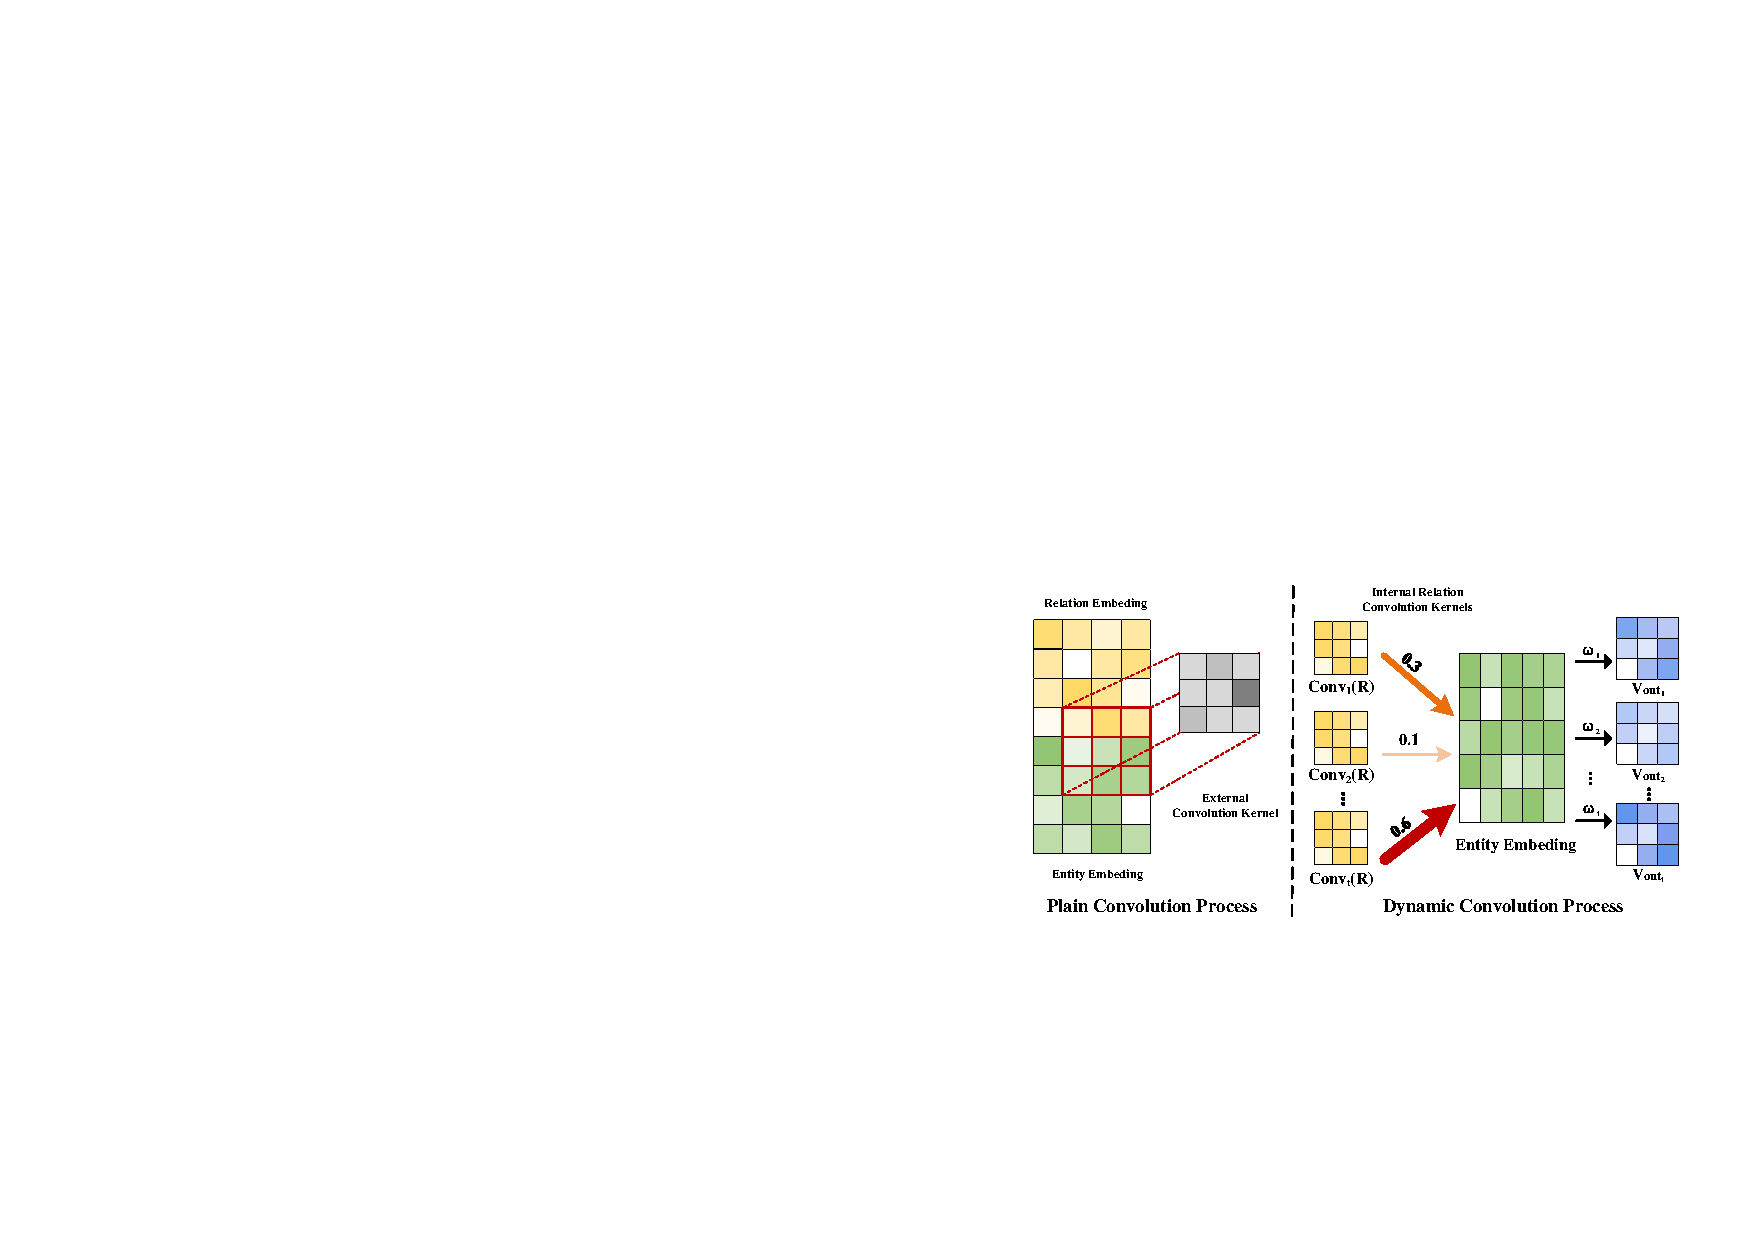
\includegraphics[width=\linewidth]{figure/motivation.pdf}
\caption{Schematic diagram of dynamic convolution and traditional plain convolution process. Dynamic convolution using multiple internal relation convolution kernels differs from the external convolution kernels in plain convolution.}
\label{fig:motivation}
\end{figure}
% \vspace{-1cm}

In this paper, we analyze the advantages and challenges of existing state-of-the-art convolutional embedding methods and propose a novel dynamic convolutional knowledge graph embedding model ConvD, as shown in Figure~\ref{fig:motivation}. ConvD first reshapes the relation vectors into multiple internal convolution kernels to directly extract the entity embedding feature information and improve the degree of model feature interaction. At the same time, the attention mechanism is introduced to calculate the correlation between entity embeddings and relation embeddings, and the adaptive dynamic convolution kernel weight vector is constructed. It should be noted that the dimension of the weight vector of ConvD will be consistent with the number of internal relational convolution kernels and adaptively and dynamically adjusted during the training process. Through this attention enhanced dynamic convolutional interaction, ConvD enables each relational convolution kernel to be effectively and rationally utilized, highlighting the critical feature information and alleviating the interference of useless information. Entity embeddings and relation embeddings can also be realized to interact effectively and adequately, significantly improving the expressive power of the model. Furthermore, a priori knowledge optimization strategy is designed for the traditional attention mechanism to further improve the accuracy of the weight coefficients in the dynamic convolution process. Notably, we construct a two-dimensional priority matrix based on the prior probability of entity-relation pairs in a KG. The higher the prior probability of an entity-relation pair, the higher the attention weight should be assigned to the pair in the dynamic convolution to improve the rationality of capturing the feature interaction information in the knowledge embedding process. In addition, ConvD also has better robustness than the existing convolutional embedding methods, which will be justified in the experimental section. Our contributions are summarized as follows:
\begin{itemize}
    \item We propose a novel dynamic convolutional embedding model ConvD for knowledge graph completion, which directly reshapes the relation embeddings into multiple internal convolution kernels and can effectively enhance feature interactions to improve model performance.
    \item We design an attention mechanism optimized by priori knowledge, which can assign different contribution weight coefficients to multiple relation convolution kernels for dynamic convolution further to improve the rationality in the feature extraction process.
    \item Extensive experiments on various datasets show that the ConvD model consistently outperforms state-of-the-art baseline methods, with an average improvement of 11.30\% to 16.92\% for all model evaluation metrics. Ablation experiments validate the effectiveness of the component modules of our proposed model.
\end{itemize}



\section{Related Work}
Existing knowledge graph embedding methods can be classified into three categories: translation distance models, semantic matching models, and neural network models.

\subsection{Translation Distance Models}
TransE~\cite{TransE} is a pioneering work in this field and has profoundly impacted subsequent developments. This model conceives the embedding space as a translation space, representing relation vectors as translation operations between entity vectors. TransH~\cite{TransH}, building upon TransE, projects entity vectors onto relation-specific hyperplanes to better distinguish similarity between different relations. TransR~\cite{TransR}, an extension of TransE and TransH, leverages relation-specific mapping matrices to capture distinct semantics between entities and relations, thereby offering improved relational representations. TransD~\cite{TransD} introduces diverse vector spaces to handle entities and relations separately, enabling an adequate representation of relation semantics. RotatE~\cite{RotatE}, on the other hand, is a rotation-based model that presents rotational operations to the complex vector model. This innovation permits entity and relation vector rotations on the complex plane, facilitating the capture of more prosperous angular relationships between triples. Typically, these models use relational embedding as a bridge for entity transformation, which has the advantages of simplicity, intuition, and computational efficiency. However, research indicates their limitations in terms of expressive power and their inapplicability to non-Euclidean spaces.

\subsection{Semantic Matching Models}
RESCAL~\cite{RESCAL} employs low-rank tensor decomposition to factorize the relation matrix into two low-rank matrices for learning vector representations of entities and relations. DistMult~\cite{DistMult} assumes symmetric relations and sets the relation matrix as a diagonal matrix. Unlike the RESCAL model, DistMult improves computational efficiency while significantly reducing the parameter count. HolE~\cite{HolE} implements a new convolution operation via Hadamard product as well as Fourier transform for defining semantic relations between entities and relations. SimplE~\cite{SimplE} employs structured embedding techniques to capture compositional information between entities and relations, effectively modeling intricate semantic details. ComplEx~\cite{ComplEx} can be considered a particular case of the SimplE model, which utilizes complex-valued vectors to represent entities and relations and excels at capturing the diversity and complexity of relations. TuckER~\cite{TuckER} adopts a three-dimensional tensor decomposition approach to learn vector representations of entities and relations. Models of this category are proficient in capturing complex relations between entities and relations in KGs. However, as the scale of KGs grows, the computational complexity of these models may escalate rapidly.


\subsection{Neural Network Models}
In recent years, researchers have explored knowledge graph embedding models based on neural networks, achieving state-of-the-art performance. ConvE~\cite{ConvE} employs 2D convolutions to model multi-layer non-linear features, extracting deep entity and relation embeddings features. ConvKB~\cite{ConvKB} delves into the global relationship between entries of entities and relations with identical embedding dimensions. ConvR~\cite{ConvR} models the interactions between different positions of entities and relations for the first time. R-GCN~\cite{R-GCN}, as a graph-based deep neural network model, capitalizes on the adjacency information of each entity. VR-GCN~\cite{VRGCN}, an extension of graph convolutional networks, is used for embedding nodes and relations. SACN~\cite{SACN} takes advantage of both GCN and ConvE to improve its expression ability. AcrE~\cite{AcrE} effectively enhances feature interaction by incorporating two distinct types of convolutions. InteractE~\cite{InteractE} augments interaction information by altering feature combinations, employing recurrent convolutions in the feature extraction process. HyperMLN~\cite{HyperMLN} is an advanced interpretable knowledge embedding framework that combines Markov logic networks and variational EM optimization algorithms for knowledge reasoning. HyConvE~\cite{HyConvE} combines 2D convolution and 3D convolution for joint training to capture deep interaction and inherent pattern information of entities and relations to improve model representation. Models of this category generally enhance feature extraction capabilities through efficient convolutional structures and well-designed combinations of entity and relation embedding features, and they have significant advantages in semantic feature learning.



\section{Preliminaries}
\subsection{Knowledge Graph}
Given a symbol $\mathcal{G}=\left(\mathcal{E}, \mathcal{R}, \mathcal{T} \right)$ represents the knowledge graph. Among them, $\mathcal{E}$ represents the set of entities, $\mathcal{R}$ represents the set of relations, and $\mathcal{T}$ represents the set of triples, that is, $\mathcal{T}=\{(h, r, t) \mid h, t \in \mathcal{E}, r \in \mathcal{R}\} \subseteq \mathcal{E} \times \mathcal{R} \times \mathcal{E}$.

\subsection{Knowledge Graph Completion} 
Knowledge completion is also called link prediction, which aims to predict missing entities or relations in KGs. Specifically, the entity prediction completion task is given the head (tail) entity and relation to predict the missing tail entity $(h, r, ?)$ or head entity $(?, r, t)$. The relation prediction completion task is given a head and tail entity to predict the missing relation between them, i.e., $(h, ?, t)$. Notably, the number of entities in real-world knowledge graph datasets is generally much larger than the number of relations, so the entity prediction task is much more common.

\begin{figure*}[!t]
\centering
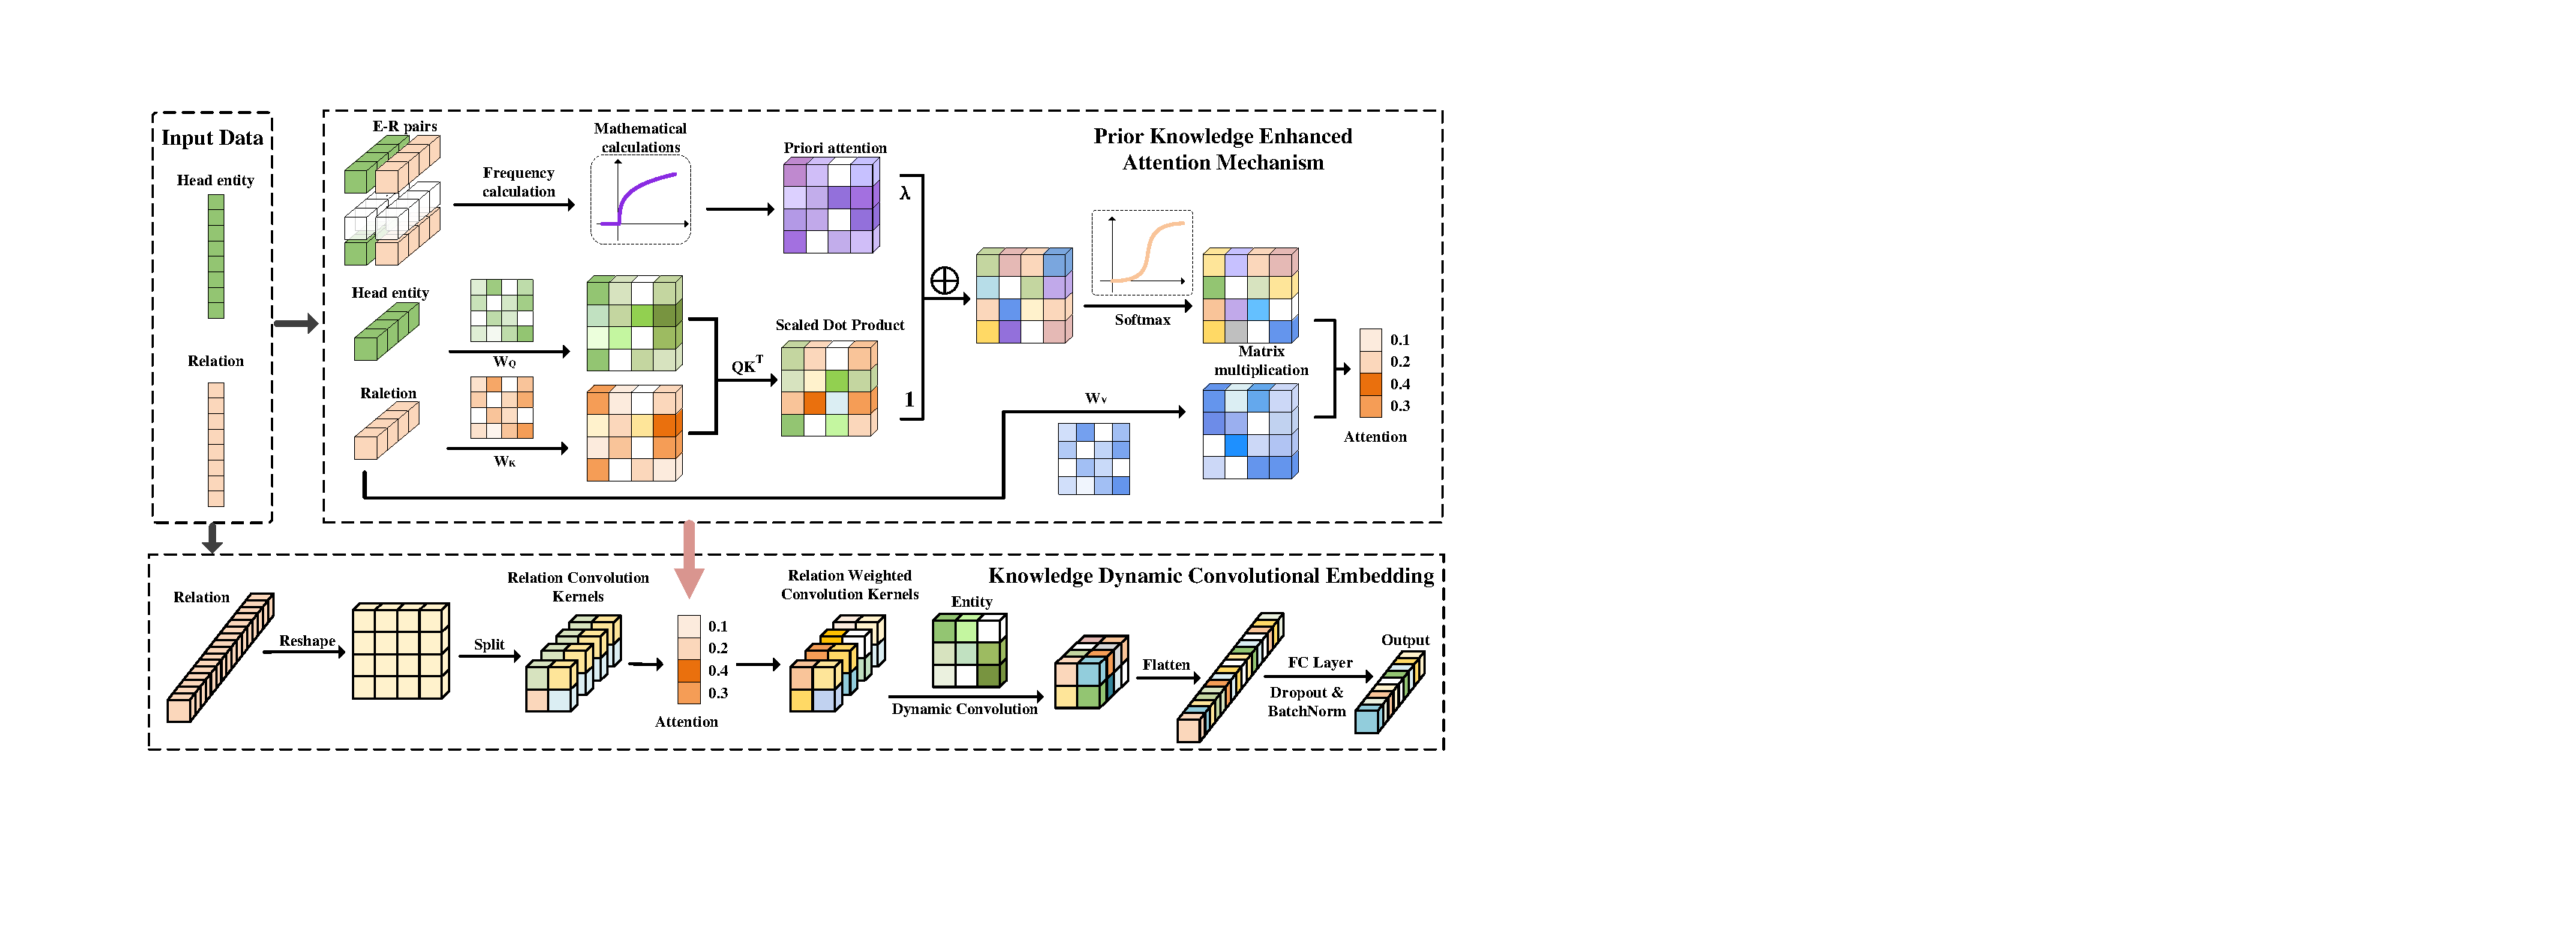
\includegraphics[width=166mm]{figure/ConvD_Model.pdf}
\caption{The overall framework of the ConvD model.}
\label{fig:model}
\end{figure*}

% \begin{figure*}[!t]
% \centering
% 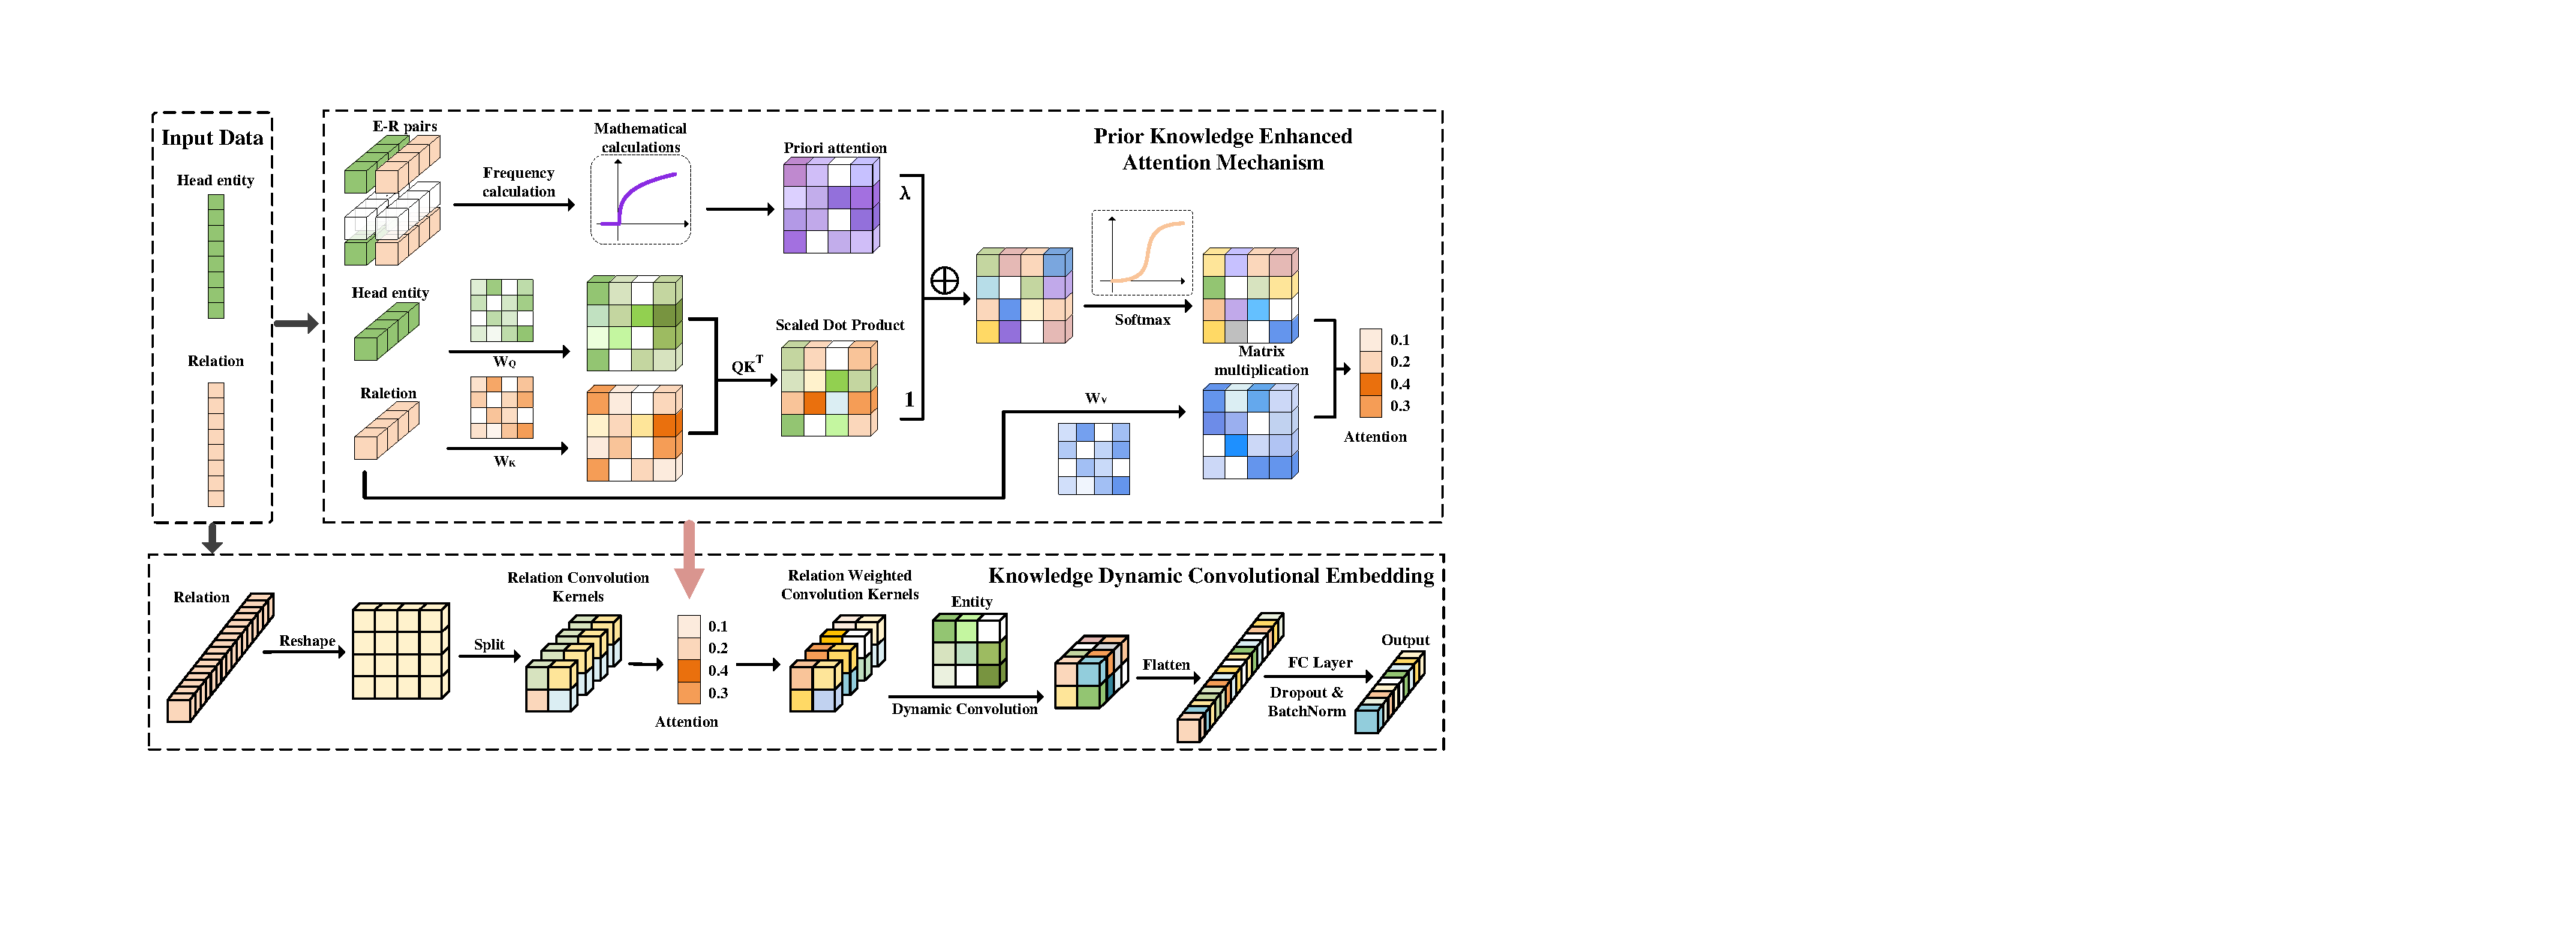
\includegraphics[width=\linewidth]{figure/ConvD_Model.pdf}
% \caption{The overall framework of the ConvD model.}
% \label{fig:model}
% \end{figure*}

\section{Methodology}
The overall framework of the ConvD model is shown in Figure~\ref{fig:model}. The final output of the model consists of two main parts. On the one hand, ConvD first reshapes the relation vectors into multiple dynamic convolution kernels with the same dimension, which directly enables the relation embeddings to extract the feature information of the entity embeddings and improves the model interaction capability. Correspondingly, each convolution kernel contributes different weights to the final output, which will be dynamically adjusted during training. On the other hand, ConvD will introduce an attention mechanism to compute the feature importance for each dynamic convolution kernel, and the weight coefficients vector dimension of the attention will be adaptively adjusted to be consistent with the number of dynamic convolution kernels. In addition, ConvD designs a priori knowledge optimization strategy for the attention mechanism to improve the accuracy of capturing the feature interaction information during the knowledge embedding process.


\subsection{Knowledge Dynamic Convolutional Embedding}
Given a knowledge triple (h, r, t), we first construct head entity embedding vectors $\boldsymbol{e}_{h} \in \mathbb{R}^{d_{e}}$ and relation embedding vectors $\boldsymbol{e}_{r} \in \mathbb{R}^{d_{r}}$. Subsequently, ConvD utilizes dynamic convolution with multiple convolution kernels to capture feature interaction information between relation embeddings and entity embeddings. The convolution kernel of ConvD is defined as: 
\begin{equation}
    \boldsymbol{\omega}_{i} = \alpha_{i} \cdot \boldsymbol{\omega}_{r}^{i}
\end{equation}
where $\alpha_{i}$ is the contribution weight factor for each convolution kernel and $\boldsymbol{\omega}_{r}^{i}$ represents each specific convolution kernel. Notably, each convolution kernel of ConvD is constructed directly from the 2D reshaping of the relation embeddings, as follows:
\begin{equation}
    \boldsymbol{\omega}_{r}^{t} = [conv_{1}(\overline{\boldsymbol{e}_{r}}); conv_{2}(\overline{\boldsymbol{e}_{r}}); ...; conv_{t}(\overline{\boldsymbol{e}_{r}})]
\end{equation}
where $conv(\cdot)$ is the convolutional construction function and $t$ is the number of the convolution kernel. The dimension of each convolution kernel $\boldsymbol{\omega}_{r}^{i}$ is set to $r_{w} \times r_{h}$, and $\overline{\boldsymbol{e}_{r}}$ is the 2D reshaping of the relation embeddings with dimension $r_{w}\sqrt{t} \times r_{h}\sqrt{t}$. Expressly, $t$ must be the square of an integer greater than zero to ensure that $\sqrt{t}$ is an integer.

ConvD uses multiple relation convolution kernels dynamically convolved with the 2D reshaping of the head entity embedding vectors. Then, the feature vector is output through a fully connected layer.
\begin{equation}
    \boldsymbol{v}_{out} = \mathrm{FC} \left (\sum_{i=1}^{t} \overline{\boldsymbol{e}_{h}} * \boldsymbol{\omega}_{i}  \right ) 
\end{equation}
where $\boldsymbol{v}_{out}$ is the output feature vector, $*$ denotes the convolution operator, and $\overline{\boldsymbol{e}_{h}} \in \mathbb{R}^{d_{w} \times d_{h}}$ represents the 2D reshaping of the head entity embedding vectors. Likewise, the dimension of the entity embedding vectors $\boldsymbol{e}_{h}$ is $d_{e}=d_{w}d_{h} \times 1$ and the dimension of the relation embedding vectors $\boldsymbol{e}_{r}$ is $d_{r}=tr_{w}r_{h} \times 1$.


\subsection{Priori Knowledge Enhanced Attention Mechanism}
The contribution weight coefficients $\alpha_{i}$ of multiple convolution kernels for dynamic convolution are crucial. ConvD introduces an attention mechanism to compute the correlation between entity embeddings and relation embeddings to construct the weight vectors of adaptive dynamic convolution kernels, as follows:
\begin{equation}
    \boldsymbol{Q}=\boldsymbol{W}_{Q}\boldsymbol{e}_{h}
\end{equation}

\begin{equation}
    \boldsymbol{K}=\boldsymbol{W}_{K}\boldsymbol{e}_{r}
\end{equation}

\begin{equation}
    \boldsymbol{V}=\boldsymbol{W}_{V}\boldsymbol{e}_{r}
\end{equation}
where $\boldsymbol{W}_{Q} \in \mathbb{R}^{d_{e} \times k}$, $\boldsymbol{W}_{K} \in \mathbb{R}^{d_{r} \times k}$, and $\boldsymbol{W}_{V} \in \mathbb{R}^{d_{r} \times t}$ are 2D projection matrices.

The attention mechanism essentially constructs a weight distribution, and this attention allocation can also come from other sources. Therefore, ConvD designs a priori knowledge optimization strategy for the traditional attention mechanism. We construct the 2D priority matrix based on the prior probability of the entity-relation pairs in the knowledge graph, and the higher the prior probability corresponding to the entity-relation pair, the stronger the correlation between them. The priority matrix is defined as:
\begin{equation}
    \boldsymbol{P}(e_{i},r_{j})=\log_{a} \left ( \mathrm{Freq}(e_{i},r_{j})+1 \right ) 
\end{equation}
where the dimension of $\boldsymbol{P}(e_{i},r_{j})$ is $d_{e} \times d_{r}$, $\mathrm{Freq}(\cdot)$ represents the frequency calculation function, and $a>1$. In particular, the priori knowledge calculation process uses logarithmic smoothing to suppress the effect of noisy data while preventing uncomputable and negative probability anomalies.

The attention mechanism enhanced by priori knowledge is as follows:
\begin{equation}
    \mathrm{Attention}(Q,K,V) = \mathrm{softmax} \left ( \frac {\boldsymbol{Q}\boldsymbol{K}^{T}}{\sqrt {d_{k}}} + \lambda \boldsymbol{P} \right ) \boldsymbol{V}
\end{equation}
where \textit{Attention} denotes the obtained attention score, $d_k$ is the dimension of the embedding vectors, and $\lambda$ is a hyperparameter to adjust the weight of the priori knowledge.

The contribution weight coefficient $\alpha_{i}$ of multiple dynamic convolution kernels is equal to $\mathrm{Attention}(Q,K,V)$.
\begin{equation}
    \alpha_{i} = \mathrm{Attention}(Q,K,V)
\end{equation}


\subsection{Joint Training}
ConvD uses a 1-N model training method to speed up computation when training model parameters, allowing training and prediction tasks to be completed in less time. Specifically, the 1-N training method computes $(h, t)$ with a set of scores for each candidate entity, and all results will be represented using a vector whose dimension is the number of entities in the dataset. The model scoring function is:
\begin{equation}
    \psi(h,r,t) = f\left( \mathrm{ReLU}\left( \boldsymbol{v}_{out} \right) \boldsymbol{W}+\boldsymbol{b} \right) \boldsymbol{e}_{t}
\end{equation}
where $\boldsymbol{v}_{out}$ is the output result of the dynamic convolution operation and $\boldsymbol{e}_{t}$ represents the object entity embedding matrix. $\boldsymbol{W}$ is the feature mapping matrix, $\boldsymbol{b}$ is the bias term, and $f(\cdot)$ denotes the \textit{sigmoid} function.

Moreover, ConvD uses three dropout layers to prevent overfitting for better training results, specifically dropout in the input data part, vector reshaping representation part, and fully connected layer part, respectively. Besides, ConvD utilizes \textit{batch normalization} to speed up the dynamic convolution operation and uses the \textit{Adam optimizer} and \textit{label smoothing} method to train the model, which adjusts the model parameters by minimizing the cross-entropy loss.
\begin{equation}
\mathcal{L}(h,r)=-\frac {1}{|\varepsilon|}\sum_{o\cup \varepsilon}y_t\log(\rho)+(1-y_t)\log(1-\rho)
\end{equation}
where $\varepsilon$ is the number of candidate entities and $\rho$ denotes the model score $\psi(h,r,t)$. The $y_t$ is a label, $y_t=1$ if $(h,r,t)$ is the correct triple, otherwise $y_t=0$.



\section{Experiments}
In this section, we describe the experimental part in detail.

\subsection{Datasets and Baselines}
\subsubsection{Datasets}
This paper uses three publicly available datasets for experiments. FB15K-237~\cite{FB15K237} and WN18RR~\cite{WN18RR} are the most common datasets in knowledge graph embedding and can be employed to compare the experimental performance of many related works. In addition, we used the DB100K~\cite{DB100K} dataset to verify the robustness of the ConvD model, which is a competitive large-scale dataset. The data size of DB100K is close to the size of the YAGO3-10 dataset. Still, the number of relations is 12.7 times more than that of YAGO3-10, which is a good choice for validating the generalization ability of the relation-centered knowledge graph embedding model. The detailed statistics of the datasets are summarized in Table~\ref{table:datasets}.
\begin{table}[h]
  \centering
  \resizebox{\linewidth}{!}{
  \begin{tabular}{cccccc}
  \toprule  
  \textbf{Dataset} & \textbf{\#Rel}  &  \textbf{\#Ent} & \textbf{\#Train} & \textbf{\#Valid} & \textbf{\#Test} \\ 
  \midrule 
  FB15K-237 & 237  &  14,541 & 272,115 & 17,535 & 20,466 \\
  WN18RR & 11  &  40,943 & 86,835 & 3,034 & 3,134 \\
  DB100K & 470  &  99,604 & 597,572 & 50,000 & 50,000 \\
  \bottomrule 
  \end{tabular}
  }
  \caption{The detailed statistics of the datasets.}
  \label{table:datasets}
\end{table}

\subsubsection{Baselines}
We compared ConvD with \textbf{25} classical and state-of-the-art baseline methods, which can be roughly divided into two categories: non-neural network models and neural network models.
\begin{itemize}
    \item \textbf{Non-Neural Network Models:} TransE~\cite{TransE}, DistMult~\cite{DistMult}, ComplEx~\cite{ComplEx}, HolE~\cite{HolE}, KBLRN~\cite{KBLRN}, Analogy~\cite{Analogy}, RUGE~\cite{RUGE}, KBGAN~\cite{KBGAN}, ComplEx-NNE-AER~\cite{NNE-AER}, RotatE~\cite{RotatE}, SEEK~\cite{SEEK}, and Sym-SEEK~\cite{SEEK}.
    \item \textbf{Neural Network Models:} Neural LP~\cite{NeuralLP}, R-GCN~\cite{RGCN}, ConvE~\cite{ConvE}, ConvKB~\cite{ConvKB}, ConvR~\cite{ConvR}, SACN~\cite{SACN}, AcrE~\cite{AcrE}, InteractE~\cite{InteractE}, DT-GCN~\cite{DT-GCN}, HyperMLN~\cite{HyperMLN}, and HyConvE~\cite{HyConvE}.
\end{itemize}


\subsection{Experimental Setup}
\subsubsection{Evaluation Settings}
We use link prediction as the proposed model evaluation task, using the common MRR and Hit@k (k taken as 1, 3, 10) as the evaluation metrics, where higher values of MRR and Hits@k indicate superior model performance. Specifically, for each triple $(h, r, t)$ of the test set, $t$ in the triple is replaced using each entity in the set of entities to generate corrupted triples, and a scoring function computes the scores of all corrupted triples. Since the constructed corrupted triples may also be correct, this paper adopts the filter setting. It is worth stating that the performance of most of the baseline methods in the experimental section is taken from the original paper, and the experimental results with ``-'' are results that were not presented in the original paper. We have only performed partial local implementations of recent models with open-source code to supplement the necessary experimental evaluation metric values.

\begin{table*}[h]
  \centering
  \resizebox{170mm}{!}{
    \begin{tabular}{c|cccc|cccc}  
        \hline
        \multirow{2}{*}{\textbf{Model}} & \multicolumn{4}{|c|}{\textbf{FB15K-237}}&\multicolumn{4}{c}{\textbf{WN18RR}} \\
        \cline{2-9}
        ~ & \textbf{MRR} & \textbf{Hit@10} & \textbf{Hit@3} & \textbf{Hit@1} & \textbf{MRR} & \textbf{Hit@10} & \textbf{Hit@3} & \textbf{Hit@1} \\
        \hline
        TransE~\cite{TransE} & 0.287 & 0.475 & 0.325 & 0.192 & 0.193 & 0.445 & 0.370 & 0.003 \\
        DistMult~\cite{DistMult} & 0.241 & 0.419 & 0.263 & 0.155 & 0.430 & 0.490 & 0.440 & 0.390 \\
        ComplEx~\cite{ComplEx} & 0.247 & 0.428 & 0.275 & 0.158 & 0.440 & 0.510 & 0.460 & 0.410 \\
        R-GCN~\cite{R-GCN} & 0.248 & 0.417 & 0.258 & 0.153 & 0.123 & 0.207 & 0.137 & 0.080 \\
        KBGAN~\cite{KBGAN} & 0.278 & 0.458 & - & - & 0.214 & 0.472 & - & - \\
        KBLRN~\cite{KBLRN} & 0.309 & 0.493 & - & 0.219 & - & - & - & - \\
        Neural LP~\cite{NeuralLP} & 0.240 & 0.362 & - & - & - & - & - & - \\
        RotatE~\cite{RotatE} & 0.338 & 0.533 & 0.375 & 0.241 & \underline{0.476} & \textbf{0.571} & \underline{0.492} & 0.428 \\
        ConvE~\cite{ConvE} & 0.316 & 0.491 & 0.350 & 0.239 & 0.460 & 0.480 & 0.430 & 0.390 \\
        ConvR~\cite{ConvR} & 0.350 & 0.528 & 0.385 & 0.261 & 0.475 & 0.537 & 0.489 & 0.443  \\
        ConvKB~\cite{ConvKB} & \underline{0.396} & 0.517 & - & - & 0.249 & 0.524 & 0.417 & 0.057 \\
        SACN~\cite{SACN} & 0.350 & 0.540 & - & 0.260 & 0.463 & 0.534 & 0.478 & 0.429 \\
        DT-GCN~\cite{DT-GCN} & 0.321 & 0.430 & 0.278 & 0.167 & 0.322 & 0.471 & 0.340 & 0.193 \\ 
        InteractE~\cite{InteractE} & 0.354 & 0.535 & - & 0.263 & 0.463 & 0.528 & - & 0.430 \\
        AcrE~\cite{AcrE} & 0.358 & \underline{0.545} & \underline{0.393} & \underline{0.266} & 0.463 & 0.534 & 0.478 & 0.429 \\        
        HyperMLN~\cite{HyperMLN} & 0.386 & 0.513 & 0.379 & 0.245 & 0.435 & 0.521 & 0.461 & 0.410 \\
        HyConvE~\cite{HyConvE} & 0.339 & 0.458 & - & 0.212 & 0.461 & 0.534 & - & \underline{0.432} \\
        \hline
        \textbf{ConvD(Ours)} & \textbf{0.409} & \textbf{0.588} & \textbf{0.447} & \textbf{0.320} & \textbf{0.479} & \underline{0.554} & \textbf{0.495} & \textbf{0.447} \\
        \hline
    \end{tabular}
  }
  \caption{Link prediction results for FB15k237 and WN18RR. The best results are in boldface and the second best are underlined. Experimental results with ``-'' are those results that were not presented in the original paper.}
  \label{table:FB15B237-WN18RR}
\end{table*}


\subsubsection{Parameter Settings}
The ConvD model is implemented on the PyTorch architecture. We set the batch size of each training to 128, the initial learning rate to 0.003, and the label smoothing coefficient to 0.1, and use grid search to optimize the hyperparameter combinations. Furthermore, the dimension of the entity embeddings are tuned in the range of $d_{e} \in \{100, 150, 200, 250, 300\}$, the convolution kernel sizes are tuned in the range of $r_{w} \times r_{h} \in \{3 \times 3, 4 \times 4, 5 \times 5\}$, and the priori knowledge weighting coefficients are tuned in the range of $\lambda \in \{0.1, 0.2, 0.3\}$. In addition, all dropout parameter values, i.e., the data input dropout $\rho_{1}$, the vector reshaping representation dropout $\rho_{2}$, and the fully connected layer dropout $\rho_{3}$, are tuned in $\{0.1, 0.2, 0.3, 0.4, 0.5, 0.6\}$. On each dataset, we select the optimal hyperparameter configuration with the highest MRR on the validation set within 200 epochs and report its performance on the test set.


\subsection{Link Prediction Results}
The results of link prediction experiments of our proposed model on FB15-237 and WN18RR datasets are shown in Table~\ref{table:FB15B237-WN18RR}. From the experimental results, ConvD performs better than the optimal baseline and has better generalization ability. Specifically, ConvD improves MRR by 3.28\%, Hit@10 by 7.89\%, Hit@3 by 13.74\%, and Hit@1 by 20.30\% over the optimal baseline method on the FB15K-237 dataset. The average improvement across all evaluation metrics is 11.30\%. And ConvD is generally superior to the optimal baseline method on the WN18RR dataset. As stated in the ConvE~\cite{ConvE} and InteractE~\cite{InteractE} papers, the WN18RR dataset has a very low average relation-specific in-degree, which is well suited for shallow models, and it is difficult for deep models to achieve superior performance. Notably, ConvD belongs to the deep models and has the best performance on the WN18RR dataset, which is a difficult achievement to reach. Concretely, compared with ConvE on the WN18RR dataset, ConvD improves MRR by 3.46\%, Hit@10 by 15.42\%, Hit@3 by 15.12\%, and Hit@1 by 14.62\%. The average improvement across all evaluation metrics is 12.16\%. 

\begin{table}[h!]
    \centering
    \resizebox{\linewidth}{!}{
        \begin{tabular}{c|cccc}  
            \toprule
            \multirow{2}{*}{\textbf{Model}} & \multicolumn{4}{c}{\textbf{DB100K}}\\
            \cmidrule(lr){2-5}
            & \textbf{MRR} & \textbf{Hit@10} & \textbf{Hit@3} & \textbf{Hit@1} \\
            \midrule
            TransE & 0.111 & 0.270 & 0.164 & 0.016 \\
            DistMult & 0.233 & 0.448 & 0.301 & 0.115 \\
            HolE & 0.260 & 0.411 & 0.309 & 0.182 \\
            ComplEx & 0.242 & 0.440 & 0.312 & 0.126 \\
            Analoge & 0.252 & 0.427 & 0.323 & 0.142 \\
            RUGE & 0.246 & 0.433 & 0.325 & 0.129 \\
            ComplEx-NNE-AER & 0.306 & 0.418 & 0.334 & 0.244 \\
            Sym-SEEK & 0.306 & 0.462 & 0.343 & 0.225 \\
            SEEK & 0.338 & 0.467 & \underline{0.370} & \underline{0.268} \\
            AcrE & 0.413 &  0.588 & 0.472 & 0.314 \\
            % ConvE & - & - & - & - \\
            DT-GCN & 0.287 & 0.427 & 0.311 & 0.187 \\
            % ConvR & - & - & - & - \\
            HyperMLN & 0.319 & 0.514 & 0.360 & 0.221 \\
            HyConvE & \underline{0.347} & \underline{0.549} & 0.349 & 0.245 \\
            \bottomrule
            \textbf{ConvD(Ours)} & \textbf{0.414} & \textbf{0.607} & \textbf{0.467} & \textbf{0.299} \\
            \bottomrule
        \end{tabular}
    }
    \caption{Link prediction results for DB100K. The best results are in boldface and the second best are underlined. All experimental results are obtained locally.}
    \label{table:DB100K}
\end{table}

% \begin{table*}[h!]
%   \begin{center}
%   \resizebox{\linewidth}{!}{
%     \begin{tabular}{c|cccc|cccc}  
%         \hline
%         \multirow{2}{*}{\textbf{Model}} & \multicolumn{4}{|c|}{\textbf{FB15K-237}}&\multicolumn{4}{c}{\textbf{WN18RR}} \\
%         \cline{2-9}
%         ~ & \textbf{MRR} & \textbf{Hit@10} & \textbf{Hit@3} & \textbf{Hit@1} & \textbf{MRR} & \textbf{Hit@10} & \textbf{Hit@3} & \textbf{Hit@1} \\
%         \hline
%         w/o Priori Knowledge & .403(-1.47\%) & .575(-2.21\%) & .434(-2.91\%) & .312(-2.50\%) & .473(-1.25\%) & .541(-2.35\%) & .482(2.63\%) & .440(-1.57\%) \\
%         w/o Attention  & .365(-10.76\%) & .534(-9.18\%) & .397(-11.19\%) & .274(-14.38\%) & .385(-19.62\%) & .467(-15.70\%) & .458(-7.48\%) & .353(-21.03\%) \\
%         w/o Priori\&Attention & .358(-12.47\%) & .529(-10.03\%) & .387(-13.42\%) & .267(-16.56\%) & .359(-25.05\%) & .449(-18.95\%) & .438(-11.52\%) & .325(-27.29\%) \\
%         \hline
%         \textbf{ConvD} & \textbf{.409} & \textbf{.588} & \textbf{.447} & \textbf{.320} & \textbf{.479} & \textbf{.554} & \textbf{.495} & \textbf{.447} \\
%         \hline
%     \end{tabular}\\
%      }
%  \end{center}
%  \caption{Results of ablation study.}
%  \label{table:ablation study}
% \end{table*}

\begin{table*}[h!]
  \resizebox{\linewidth}{!}{
    \begin{tabular}{c|cccc|cccc}  
        \hline
        \multirow{2}{*}{\textbf{Model}} & \multicolumn{4}{c|}{\textbf{FB15K-237}} & \multicolumn{4}{c}{\textbf{WN18RR}} \\
        \cline{2-9}
        ~ & \textbf{MRR} & \textbf{Hit@10} & \textbf{Hit@3} & \textbf{Hit@1} & \textbf{MRR} & \textbf{Hit@10} & \textbf{Hit@3} & \textbf{Hit@1} \\
        \hline
        w/o Priori Knowledge & 0.403 & 0.575 & 0.434 (\SI{-2.91}{\percent}) & 0.312 & 0.473 & 0.541 & 0.482 (\SI{-2.63}{\percent}) & 0.440 \\
        w/o Attention  & 0.365 & 0.534 & 0.397 & 0.274 (\SI{-14.38}{\percent}) & 0.385 & 0.467 & 0.458 & 0.353 (\SI{-21.03}{\percent}) \\
        w/o Priori\&Attention & 0.358 & 0.529 & 0.387 & 0.267 (\SI{-16.56}{\percent}) & 0.359 & 0.449 & 0.438 & 0.325 (\SI{-27.29}{\percent}) \\
        \hline
        \textbf{ConvD} & \textbf{0.409} & \textbf{0.588} & \textbf{0.447} & \textbf{0.320} & \textbf{0.479} & \textbf{0.554} & \textbf{0.495} & \textbf{0.447} \\
        \hline
    \end{tabular}
  }
 \caption{Results of ablation study. The maximum percentage of performance reduction is labeled for each set of experiments.}
 \label{table:ablation-study}
\end{table*}

% \begin{figure*}[h!]
%   \centering
%   \label{fig:dynamic Convolution}
% 	\subfigure[MRR]{ \label{jf:mrr} 
% 		\includegraphics[width=0.22\textwidth, height=0.2\textwidth]{JF_mrr.pdf}}
% 	\quad
% 	\subfigure[Hit@1]{ \label{jf:hit1} 
% 		\includegraphics[width=0.22\textwidth, height=0.2\textwidth]{JF_hit1.pdf}}
% 	\quad
% 	\subfigure[Hit@3]{ \label{jf:hit3} 
% 		\includegraphics[width=0.22\textwidth, height=0.2\textwidth]{JF_hit3.pdf}}
% 	\quad
% 	\subfigure[Hit@10]{ \label{jf:hit19} 
% 		\includegraphics[width=0.22\textwidth, height=0.2\textwidth]{JF_hit10.pdf}}
%     \caption{Results of dynamic convolution removal of different percentages of convolution kernels.}
% \end{figure*}

% \begin{figure*}[h!]
%   \centering
%   \label{fig:dynamic Convolution}
% 	\subfigure[FB15K-237]{
% 		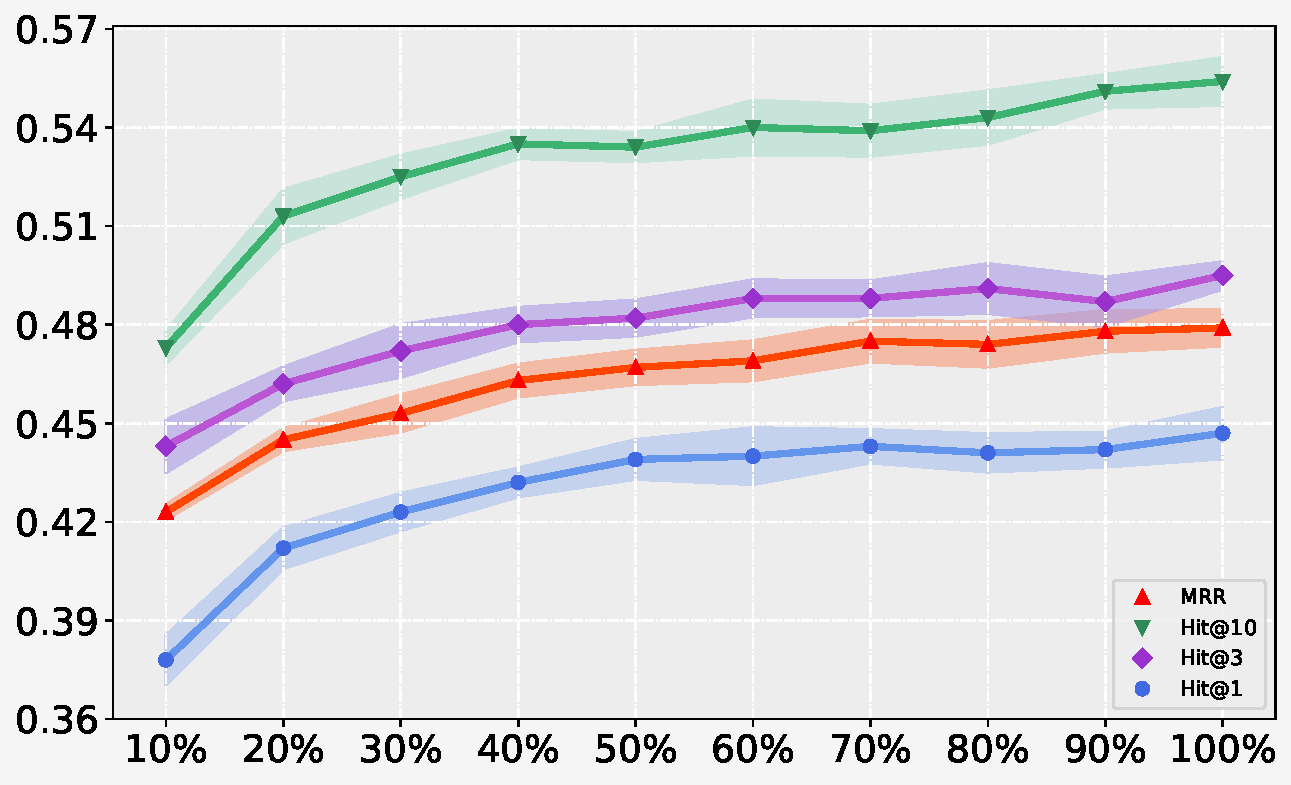
\includegraphics[width=0.40\textwidth, height=0.27\textwidth]{figure/WN18RR.pdf}}
% 	\quad
% 	\subfigure[WN18RR]{
% 		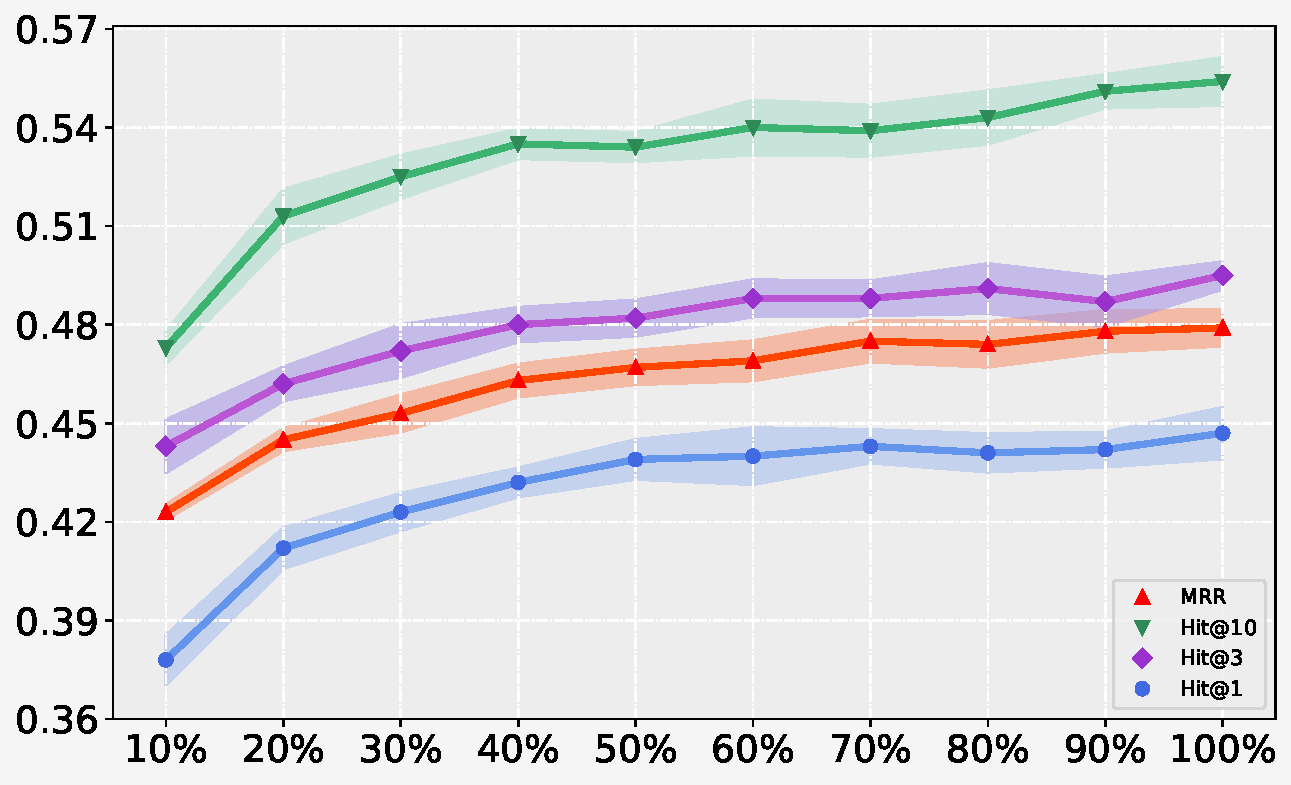
\includegraphics[width=0.40\textwidth, height=0.27\textwidth]{figure/WN18RR.pdf}}
%     \caption{Results of dynamic convolution removal of different percentages of convolution kernels.}
% \end{figure*}

The results of link prediction experiments of our proposed model on DB100K datasets are shown in Table~\ref{table:DB100K}. The experimental results show that the proposed model significantly outperforms the optimal baseline model, proving ConvD has a strong generalization ability on larger-scale datasets. It is worth noting that DB100K is a larger-scale dataset with more relations, which is an experimental validation with practical applications for knowledge graph embedding focusing on relations. Specifically, ConvD improves MRR by 19.31\%, Hit@10 by 10.56\%, Hit@3 by 26.22\%, and Hit@1 by 11.57\% over the optimal baseline method on the DB100K dataset. The average improvement across all evaluation metrics is 16.92\%.

Experiments on different public datasets demonstrate the superiority of our proposed model, with ConvD improving performance by an average of 11.30\% to 16.92\% across all model evaluation metrics. The ConvD can capture better feature interaction information on datasets with very low average relation-specific in-degree to achieve better performance due to the direct reshaping of relation embeddings into internal convolution kernels. In addition, ConvD can also dynamically and adaptively adjust the contribution weight coefficients of multiple convolution kernels on large-scale datasets with more relations through the priori knowledge-optimized attention mechanism to ensure better generalization ability and performance.


\begin{figure}[h!]
  \centering
	\subfigure[FB15K-237]{
		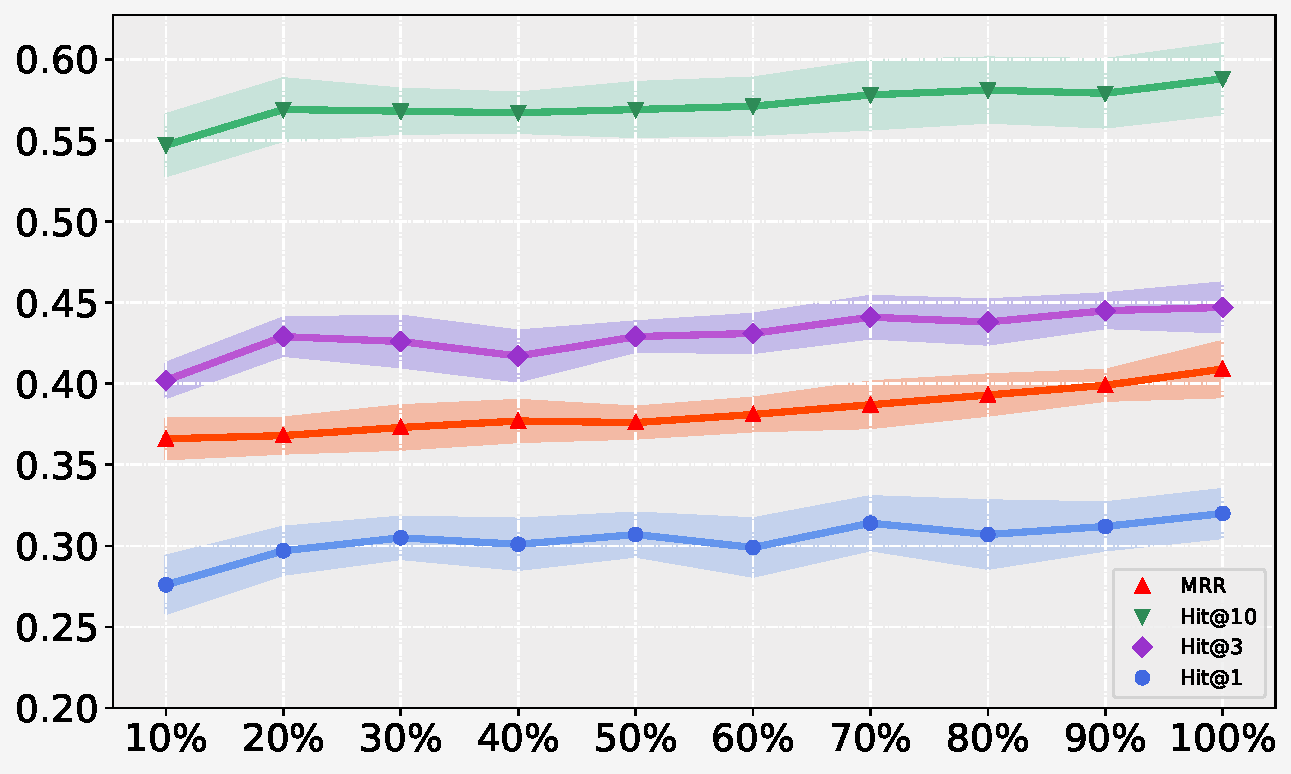
\includegraphics[width=0.42\textwidth, height=0.25\textwidth]{figure/FB15K237.pdf}}
	\\
	\subfigure[WN18RR]{
		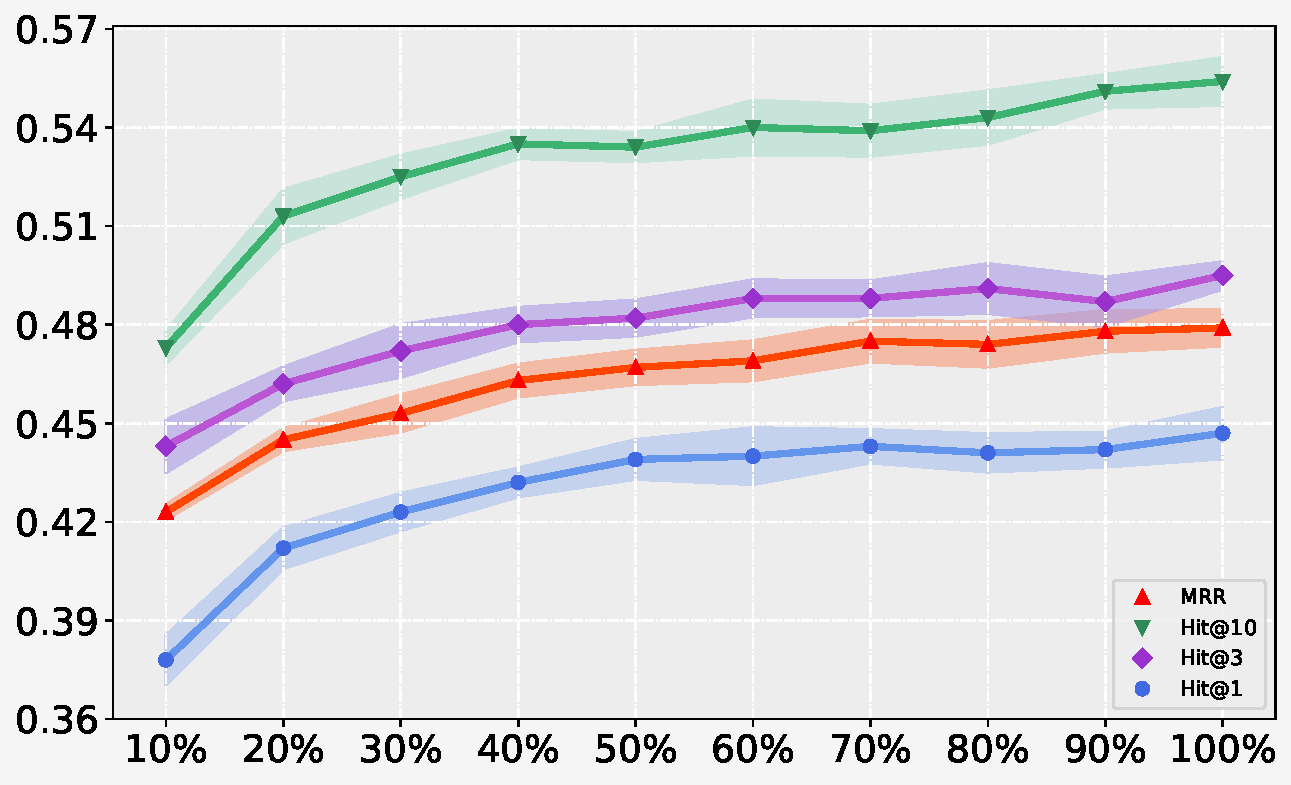
\includegraphics[width=0.42\textwidth, height=0.25\textwidth]{figure/WN18RR.pdf}}
    \caption{Results of dynamic convolution removal of different percentages of convolution kernels.}
  \label{fig:dynamic convolution}
\end{figure}


\subsection{Ablation Study}
Ablation experiment is a necessary research content to verify the function of each module of the knowledge embedding model. We select two standard knowledge graph datasets, FB15K-237 and WN18RR, and conduct ablation experiments using the same hyperparameters as the link prediction experiments, the results of which are shown in Table~\ref{table:ablation study}. It should be noted that the DB100K dataset is large, and the model training iteration rounds are long, so an ablation study is not performed on it, but this does not affect the validity of the conclusions of the ablation experiments. Especially, we perform three different sets of ablation experiments, namely ConvD without a priori knowledge optimization strategy (w/o Priori Knowledge), ConvD without the attention mechanism (w/o Attention), and ConvD without the priori knowledge-optimized attentional mechanism (w/o Priori\&Attention).

From the experimental results, it can be seen that all the model evaluation metrics of ConvD (w/o Priori Knowledge) have performance reduction ranging from 1.47\% to 2.91\% on the FB15K-237 dataset and from 1.25\% to 2.63\% on the WN18RR dataset. ConvD (w/o Attention) all model evaluation metrics degraded performance by 9.18\% to 14.38\% on the FB15K-237 dataset and 7.48\% to 21.03\% on the WN18RR dataset. ConvD (w/o Priori\&Attention) all model evaluation metrics degraded performance by 10.03\% to 16.56\% on the FB15K-237 dataset and 11.52\% to 27.29\% on the WN18RR dataset. Overall, the results of the ablation experiments indicate that each of the ConvD constituent modules is critical. The attention mechanism has a somewhat more significant impact on model performance than the priori knowledge optimization strategy. The ablation experiments on the WN18RR dataset, which has a very low average relation-specific in-degree, demonstrate the superiority of the attention enhanced multiple relation convolution kernels for the ConvD model from another perspective.


\subsection{Effect of Dynamic Convolution}
The dynamic convolution part of ConvD is coupled to the attention mechanism, so the ablation experiments provide some evidence for the effectiveness of the dynamic convolution module. In addition, the number of convolution kernels for dynamic convolution is also an important parameter to focus on, and this subsection explores the performance impact of the number of dynamic convolution kernels on knowledge embedding. We select two standard knowledge graph datasets, FB15K-237 and WN18RR, and conduct the effects of dynamic convolution experiments using the same hyperparameters as the link prediction experiments, the results of which are shown in Figure~\ref{fig:dynamic convolution}. It can be observed that the variation of each model evaluation metric on the FB15K-237 dataset is slight. On the WN18RR dataset, the ConvD model is essentially stable when the number of dynamic convolutional kernels is retained above 60\%, and a significant performance decay can be observed when the number of dynamic convolutional kernels is maintained below 60\%. Since the number of relations in the WN18RR dataset is much less than that in the FB15K-237 dataset and the average relation-specific in-degree is very low, it relies heavily on the number of relation-aware dynamic convolution kernels constructed by ConvD to enhance the model feature extraction capability. 



\section{Conclusion}
In this paper, we propose a dynamic convolutional embedding method ConvD for knowledge graph completion, which mainly constructs multiple relation-aware internal convolution kernels to increase feature interactions. Additionally, ConvD uses an attention mechanism optimized with priori knowledge to assign different weight coefficients to multiple relation convolution kernels, improving the model's generalization ability. Experiments on different datasets show that our proposed model has consistent and significant superiority and robustness over other state-of-the-art methods.



% \section{Acknowledgments}
% Thank you for reading these instructions carefully. We look forward to receiving your electronic files!
% \bigskip
% \noindent Thank you for reading these instructions carefully. We look forward to receiving your electronic files!

\bibliography{aaai24}

\end{document}
